\section{Qualitätsszenarien (DH)}
In diesem Kapitel werden Szenarien vorgestellt, mit denen die Qualitätsziele beispielhaft verdeutlicht werden. 

\subsection{Qualitätsbaum}
Abbildung \ref{fig:Qualitaetsbaum} liefert einen Überblick über die Qualitätsmerkmale und welche Szenarien ihnen zugeordnet sind.
\begin{figure}[htbp]
	\centering
		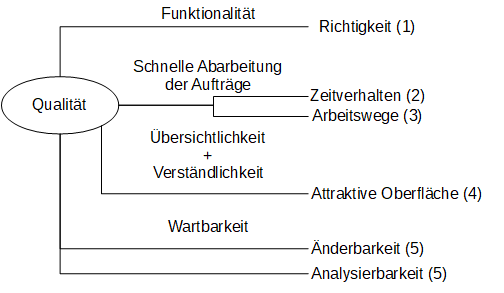
\includegraphics[width=0.50\textwidth]{figures/Qualitaetsbaum.PNG}
	\caption{Qualitätsbaum}
	\label{fig:Qualitaetsbaum}
\end{figure}

\subsection{Bewertungsszenarien}
Die Qualitätsszenarien sind:
\begin{enumerate}
	\item Die Eingabemasken filtern falsche oder fehlende Eingaben heraus und zeigen Warnungen an, so dass der Anwender die Eingaben korrigieren kann, bevor die Anwendung die Eingaben verarbeitet.
	\item Die Listen sollen innerhalb von Millisekunden angezeigt werden. Die Buchung eines Buches für alle Schüler einer Klasse soll innerhalb von 2 Sekunden erfolgt sein.
	\item Zusammengehörende Funktionen sollen über eine gemeinsame Oberfläche ausgeführt werden können. Hiermit sollen unnötige Mausklicks vermieden werden.
	\item Die Oberflächen sind ansprechend, Aufgaben werden erläutert und die Darstellung ist benutzerfreundlich (siehe Anhang \ref{USABILITY_ASPEKTE}).
	\item Der Sourcecode der Anwendung ist dokumentiert und unter Verwendung von Coding Conventions implementiert (siehe Kapitel \ref{KONVENTIONEN}). Des Weiteren ist der Code so organisiert, dass Änderungen möglichst einfach durchgeführt werden können.
\end{enumerate}